\chapter{Déroulement du projet}

  \section{Diagramme de Gantt prévisionnel}

\begin{figure}[!ht]
         \centering
         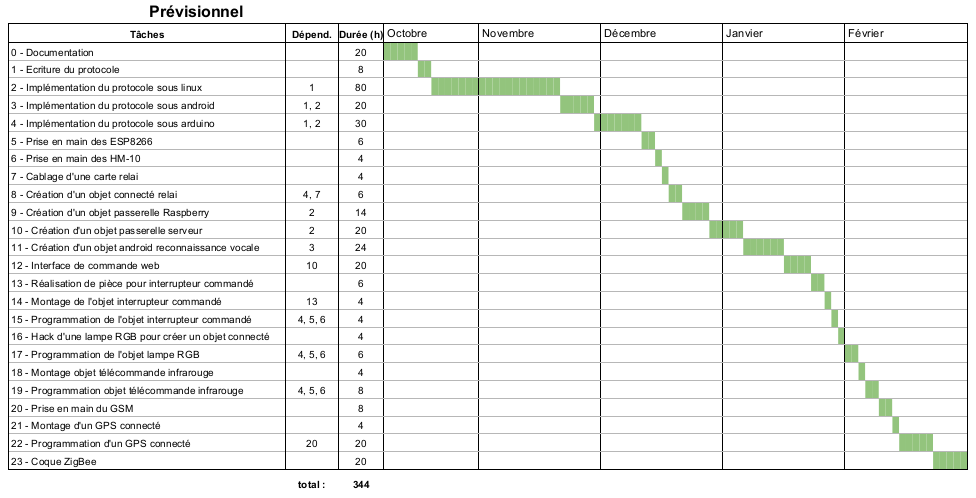
\includegraphics[width=1.1\textwidth]{img/gantt_prev}
         \caption{Diagramme de Gantt prévisionnel}
         \label{Gantt_prev}
\end{figure}

On peut voir que la durée du projet était étalonnée à 344H au total, beaucoup de tâches ont été rajouté si 
jamais du temps était trouvé.

  \section{Diagramme de Gantt réel}
	
\begin{figure}[!ht]
         \centering
         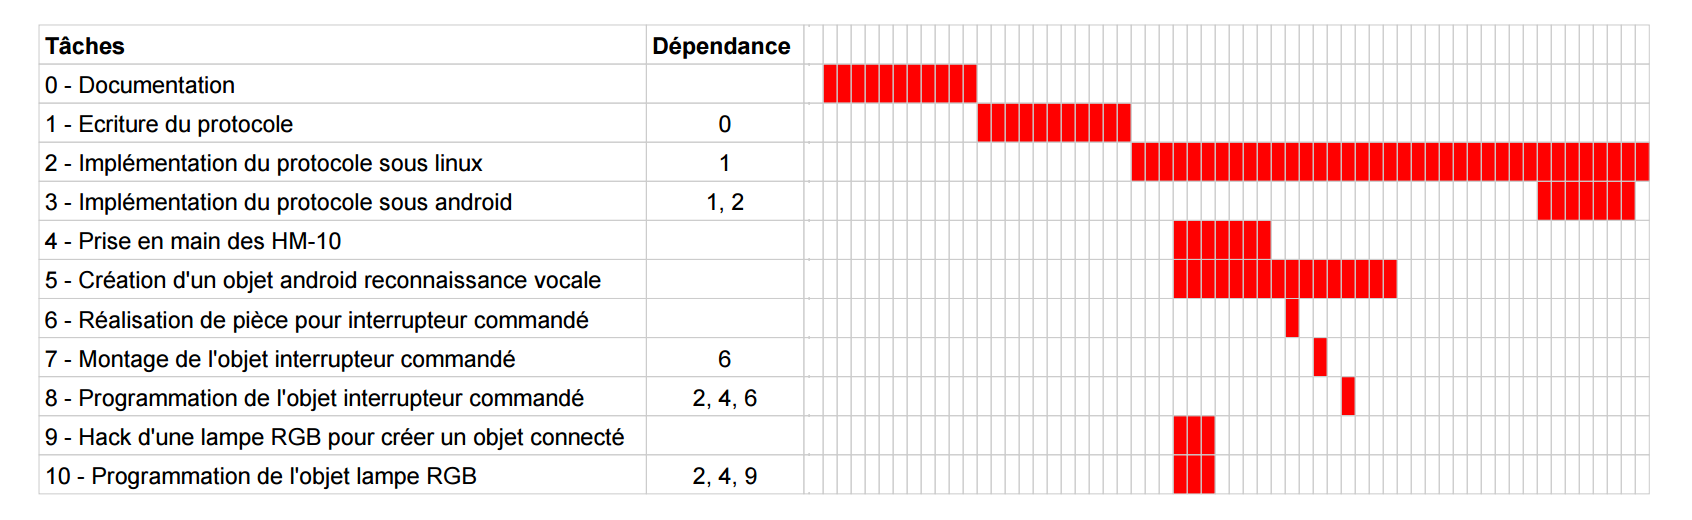
\includegraphics[width=1.1\textwidth]{img/gantt_reel}
         \caption{Diagramme de Gantt reel}
         \label{Gantt_reel}
\end{figure}

On peut voir qu'il y a énorméments moins de tâches dans le Gantt réel, que dans le Gantt prévisionnel. Cela 
vient du fait qu'il y a énorméments de choses que nous pensions réalisable plus rapidement.


